\documentclass{beamer}

\usepackage{amssymb,amsmath,verbatim,graphicx,microtype,units,booktabs,upquote,xcolor,siunitx,csquotes,fancyvrb,newverbs,wrapfig,multicol}
\hypersetup{
            colorlinks = true,
            linkcolor = blue,
            urlcolor  = blue,
            citecolor = blue,
            anchorcolor = blue
}

\title{Fundamentals of Git}
\subtitle{Missouri Satellite Team}
\author{Presented by: Illya Starikov}
\date{ }

\newcommand{\shellcmd}[1]{\texttt{\colorbox{gray!30}{#1}}}

\definecolor{cverbbg}{gray}{.7}
\newenvironment{lcverbatim}
 {\SaveVerbatim{cverb}}
 {\endSaveVerbatim
  \flushleft\fboxrule=0pt\fboxsep=.5em
  \scriptsize
  \colorbox{cverbbg}{%
    \makebox[\dimexpr\linewidth-2\fboxsep][l]{\BUseVerbatim{cverb}}%
  }
  \endflushleft
}

\newcommand{\hugeslide}[1]{
\begin{frame}[plain,c]
    \centering {\usebeamerfont*{frametitle} \usebeamercolor[fg]{frametitle}\fontsize{40}{50}\selectfont #1}
\end{frame}
}
\begin{document}
\begin{frame}
    \maketitle
\end{frame}

\begin{frame}
    \frametitle{Getting Started}

    There'll be some setting up before you can start using git. It'll depend on your operating system --- you can refer to the installation guide
    \href{https://git-scm.com/book/en/v2/Getting-Started-Installing-Git}{here}.
    Below are the more popular methods of installation.

    \begin{description}
        \item[macOS] \shellcmd{brew install git}\footnote{Or whatever hip package manager you use.}
        \item[Linux] Depends on your distro. If Ubuntu use \shellcmd{sudo apt-get install git-all}, if Arch Linux then \shellcmd{pacman -S git}, if others refer \href{https://git-scm.com/download/linux}{here}.
        \item[Windows] Download a \texttt{.exe} from \href{https://git-scm.com/download/win}{here}.
    \end{description}

\end{frame}

\begin{frame}
    \frametitle{What is Git?}

    \begin{multicols}{2}
        \begin{itemize}
            \item Git is nothing more than Directed Acyclic Graph of objects compressed and identified by an SHA-1 hash. % What?
            \item Git works in snapshots, not differences. % Meaning when you commit (or save), you save a mini filesystem at the time of commit. This makes going through and seeing changes very easy
                \item Git is local. % Changes can be saved and continue your work no matter where you are. You can't receive/transmit changes from the remote, central repository, but you can continue your work (when you are ready to pull changes from central repo, it'll merge).
            \item Git has data integrity. % That's the SHA-1 hash. All your snapshots are referred to by a checksum.
            \item Git is parallelizable. % Meaning hundreds of people can work on hundreds different versions of the repository, and it'll still work.
        \end{itemize}

        \begin{center}
            
\includegraphics[width=0.35\textwidth]{xkcd}
        \end{center}
    \end{multicols}
\end{frame}

\begin{frame}
    \frametitle{The Five Stages of Git}

    \begin{enumerate}
        \item Working Directory % This is the local repository. The changes and modification you make are in this stage, until you 'add' (i.e. specifically say these are the files whos changes you want to `commit') them.
        \item Staging Area % When files are 'added', they are in the staging area, you ready for you to say `these are the changes I made'.
        \item Git Directory % After `committing' (nothing more than saying I made these changes, here's what's different), they are updated in the git databases
        \item $\cdots$
        \item Profit % fuck yeah!
    \end{enumerate}
\end{frame}

\begin{frame}
    \frametitle{\shellcmd{Git}ting Good}

    If the ``stages'' didn't make sense, that's alright. It's better to go through a workflow as apposed to the formalities.

    \begin{enumerate}
        \item Start a new repository with \shellcmd{git init} % this creates your working directory
        \item Work on project in bite sized chunks, and add files that were changed with \shellcmd{git add file(s)} % adding to the staging area
        \item Commit your changes with \shellcmd{git commit} % This transfers them to the Git directory
        \item Optionally, \shellcmd{git push} to save changes to the remote branch
        \item Of course, profit.
    \end{enumerate}
\end{frame}

\begin{frame}
    \frametitle{The Commit Message}
    This is the easiest part of git --- and also the easiest to mess up. Here are \href{http://chris.beams.io/posts/git-commit/}{seven rules of a great commit message}.
    \begin{multicols}{2}
        \begin{enumerate}
            \item Separate subject from body with a blank line.
            \item Limit the subject line to 50 characters.
            \item Capitalize the subject line.
            \item Do not end the subject line with a period.
            \item Use the imperative mood in the subject line.
            \item Wrap the body at 72 characters.
            \item Use the body to explain \textit{what} and \textit{why} vs. \textit{how}.
        \end{enumerate}

        \begin{center}
            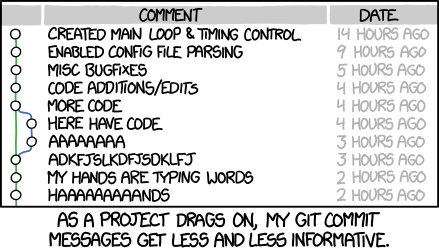
\includegraphics[width=0.45\textwidth]{xkcd-2}
        \end{center}
    \end{multicols}
\end{frame}

\begin{frame}[fragile]
    \frametitle{The Commit Message (Example)}

    \begin{lcverbatim}
Summarize changes in around 50 characters or less

More detailed explanatory text, if necessary. Wrap it to about 72
characters or so. In some contexts, the first line is treated as the
subject of the commit and the rest of the text as the body. The
blank line separating the summary from the body is critical (unless
you omit the body entirely); various tools like `log', `shortlog'
and `rebase' can get confused if you run the two together.

Explain the problem that this commit is solving. Focus on why you
are making this change as opposed to how (the code explains that).
Are there side effects or other unintuitive consequences of this
change? Here's the place to explain them.

Further paragraphs come after blank lines.

 - Bullet points are okay, too

 - Typically a hyphen or asterisk is used for the bullet, preceded
   by a single space, with blank lines in between, but conventions
   vary here
    \end{lcverbatim}
\end{frame}


\hugeslide{Demo}


\begin{frame}
    \frametitle{\shellcmd{Git}ting Better}

    Some more advanced commands to make your job easier.

    \begin{itemize}
        \item The wildcard \shellcmd{*} expands to whatever can fit a certain pattern.
        \begin{itemize}
            \item \shellcmd{git add *.cpp} stages all files with a \shellcmd{cpp} extension.
            \item \shellcmd{git add damon.*} add all document types with the name of \texttt{damon}, whether it be \shellcmd{cpp}, \shellcmd{txt}, or (unfortunately) \shellcmd{jpg}.
        \end{itemize}

        \item \shellcmd{git add -A} stages new, modified, and modified files.
        \item \shellcmd{git commit -m ``<msg>''} commits with the commit message \texttt{<msg>}. \textbf{Only use if you absolutely know what you're doing.}
    \end{itemize}
\end{frame}



\end{document}
